\documentclass[11pt, twocolumn]{article}
\usepackage{graphicx} %package to manage images
\graphicspath{ {./images/} }
\usepackage{wrapfig}
\usepackage{titlesec}
\usepackage{amsmath,amssymb,amsthm,enumerate,nicefrac,fancyhdr,hyperref,adjustbox}
\hypersetup{colorlinks=true,urlcolor=blue,citecolor=black,linkcolor=blue}
\usepackage[left=1.5cm, right=1.5cm, top=1.5cm, includehead, includefoot]{geometry}
\usepackage[dvipsnames]{xcolor}
\usepackage[d]{esvect}
\usepackage{tikz}
\usepackage{enumitem}
\usepackage{siunitx}
\usepackage{amsmath}
\allowdisplaybreaks
\usepackage[style=apa]{biblatex}
% put biblatex references in myrefs.bib, upload to root in overleaf
\addbibresource{mondrefs.bib}
% use \parencite{citation_name} to insert an in-text citation in (author, year) format

%% commands
%% useful macros [add to them as needed]
% sets
\newcommand{\C}{{\mathbb{C}}}
\newcommand{\N}{{\mathbb{N}}}
\newcommand{\Q}{{\mathbb{Q}}}
\newcommand{\R}{{\mathbb{R}}}
\newcommand{\Z}{{\mathbb{Z}}}
\newcommand{\F}{{\mathbb{F}}}
\newcommand{\Zm}{\Z_m}
\newcommand{\Zp}{\Z_p}

% bases
\newcommand{\mA}{\mathcal{A}}
\newcommand{\mB}{\mathcal{B}}
\newcommand{\mC}{\mathcal{C}}
\newcommand{\mD}{\mathcal{D}}
\newcommand{\mE}{\mathcal{E}}
\newcommand{\mL}{\mathcal{L}}
\newcommand{\mM}{\mathcal{M}}
\newcommand{\mO}{\mathcal{O}}
\newcommand{\mP}{\mathcal{P}}
\newcommand{\mS}{\mathcal{S}}
\newcommand{\mT}{\mathcal{T}}

% linear algebra
\newcommand{\diag}{\operatorname{diag}}
\newcommand{\adj}{\operatorname{adj}}
\newcommand{\rank}{\operatorname{rank}}
\newcommand{\spn}{\operatorname{Span}}
\newcommand{\proj}{\operatorname{proj}}
\newcommand{\prp}{\operatorname{perp}}
\newcommand{\refl}{\operatorname{refl}}
\newcommand{\tr}{\operatorname{tr}}
\newcommand{\nul}{\operatorname{Null}}
\newcommand{\nully}{\operatorname{nullity}}
\newcommand{\range}{\operatorname{Range}}
\renewcommand{\ker}{\operatorname{Ker}}
\newcommand{\col}{\operatorname{Col}}
\newcommand{\row}{\operatorname{Row}}
\newcommand{\cof}{\operatorname{cof}}
\newcommand{\Num}{\operatorname{Num}}
\newcommand{\Id}{\operatorname{Id}}
\newcommand{\ipb}{\langle \thinspace, \rangle}
\newcommand{\ip}[2]{\left\langle #1, #2\right\rangle} % inner products
\newcommand{\M}[2]{M_{#1\times #2}(\F)}
\newcommand{\RREF}{\operatorname{RREF}}
\newcommand{\REF}{\operatorname{REF}}
\newcommand{\cv}[1]{\begin{bmatrix} #1 \end{bmatrix}}
%\newenvironment{amatrix}[1]{\left[\begin{array}{@{}*{\numexpr#1-1}{c}|c@{}}}{\end{array}\right]}
\newcommand{\am}[2]{\begin{amatrix}{#1} #2 \end{amatrix}}

% vectors
\newcommand{\vzero}{\vv{0}}
\newcommand{\va}{\vv{a}}
\newcommand{\vb}{\vv{b}}
\newcommand{\vc}{\vv{c}}
\newcommand{\vd}{\vv{d}}
\newcommand{\ve}{\vv{e}}
\newcommand{\vf}{\vv{f}}
\newcommand{\vg}{\vv{g}}
\newcommand{\vh}{\vv{h}}
\newcommand{\vl}{\vv{\ell}}
\newcommand{\vm}{\vv{m}}
\newcommand{\vn}{\vv{n}}
\newcommand{\vp}{\vv{p}}
\newcommand{\vq}{\vv{q}}
\newcommand{\vr}{\vv{r}}
\newcommand{\vs}{\vv{s}}
\newcommand{\vt}{\vv{t}}
\newcommand{\vu}{\vv{u}}
\newcommand{\vvv}{{\vv{v}}}
\newcommand{\vw}{\vv{w}}
\newcommand{\vx}{\vv{x}}
\newcommand{\vy}{\vv{y}}
\newcommand{\vz}{\vv{z}}

% display
\newcommand{\ds}{\displaystyle}
\newcommand{\qand}{\quad\text{and}}
\newcommand{\qandq}{\quad\text{and}\quad}
\newcommand{\hint}{\textbf{Hint: }}
\newcommand*\circled[1]{\tikz[baseline=(char.base)]{
		\node[shape=circle,draw,inner sep=2pt] (char) {#1};}}

% misc
\newcommand{\area}{\operatorname{area}}
\newcommand{\vol}{\operatorname{vol}}
\newcommand{\red}[1]{{\color{red} #1}}
\newcommand{\rc}{\red{\checkmark}}

% fractions
\newcommand{\ff}[2]{\frac{#1}{#2}}

% other
\newcommand{\la}[1]{\begin{enumerate}[label=(\alph*)] #1  \end{enumerate}}
\newcommand{\dv}[1]{\vv{#1}=\cv{#1 _1\\ \vdots\\ #1 _n}}
\newcommand{\dcv}[1]{\cv{#1 _1\\ \vdots\\ #1 _n}}
\newcommand{\tbf}[1]{\textbf{#1}}
\newcommand{\ti}[1]{\textit{#1}}
\newcommand{\dt}[2]{\vv{#1} \cdot \vv{#2}}
\newcommand{\ddt}[2]{\vv{#1} \cdot \vv{#2} = \normv{#1} \normv{#2} \cos \theta}
\newcommand{\cs}[2]{\vv{#1} \times \vv{#2}}
\newcommand{\ps}[2]{\vv{#1} + \vv{#2}}
\newcommand{\ms}[2]{\vv{#1} - \vv{#2}}
\newcommand{\norm}[1]{\| #1 \|}
\newcommand{\normv}[1]{\| \vv{#1} \|}
\newcommand{\abs}[1]{| #1 |}
\newcommand{\normalisation}[1]{\frac{\vv{#1}}{\norm{\vv{#1}}}}
\newcommand{\q}{\begin{flushright} Q.E.D.\end{flushright}}
\newcommand{\projv}[2]{\proj_{\vv{#1}}\left(\vv{#2}\right)}
\newcommand{\ipv}[2]{\left\langle \vv{#1}, \vv{#2}\right\rangle}
\newcommand{\also}{\text{ and }}
\newcommand{\prpv}[2]{\prp_{\vv{#1}}(\vv{#2})}
\newcommand{\spnd}[1]{\spn \left\{\cv{#1}\right\}}
\newcommand{\spndd}[2]{\spn \left\{\cv{#1}, \cv{#2}\right\}}
\newcommand{\bm}[1]{\begin{bmatrix}#1\end{bmatrix}}
\newcommand{\ma}[1]{\begin{matrix}#1\end{matrix}}
\newcommand{\ca}[1]{\begin{cases}#1\end{cases}}
\newcommand{\ero}[1]{\text{ERO's: } \ca{#1}}
\newcommand{\rref}[1]{\RREF \left(#1\right)}
\newcommand{\reff}[1]{\REF \left(#1\right)}
\newcommand{\rankk}[1]{\rank \left(#1\right)}
\newcommand{\nullity}[1]{\nully \left(#1\right)}
\newcommand{\aug}[2]{\left[#1|#2\right]}
\newcommand{\augv}[2]{\left[#1|\vv{#2}\right]}
\newcommand{\st}{\text{ s.t. }}
\newcommand{\qef}{\begin{flushright} Q.E.F.\end{flushright}}
\newcommand{\rowm}[1]{\row(#1)}
\newcommand{\nulm}[1]{\nul(#1)}
\newcommand{\balign}[1]{\begin{align*}#1\end{align*}}
\newcommand{\sm}[3]{\begin{amatrix}{#1}{#2} #3 \end{amatrix}}
\newcommand{\smt}[1]{\begin{smatrixt} #1 \end{smatrixt}}
\renewcommand\qedsymbol{Q.E.D.}
\newcommand{\dett}[1]{\det\left(#1\right)}
\newcommand{\switch}{\leftrightarrow}
\newcommand{\prooff}{\ti{Proof. }}
\newcommand{\adjj}[1]{\adj\left(#1\right)}
\newcommand{\cae}[2]{C_{#1}(#2)}
\newcommand{\cA}[1]{\cae{A}{#1}}
\newcommand{\lam}{\lambda}
\newcommand{\elam}[1]{E_{\lam}(#1)}
\newcommand{\nulll}[1]{\nul (#1)}
\newcommand{\degg}[1]{\deg(#1)}
\newcommand{\disproof}{\ti{Disproof. }}
\newcommand{\pa}{\partial}
\newcommand{\paf}[2]{\ff{\pa #1}{\pa {#2}}}
\newcommand{\ppaf}[2]{\ff{\pa^2 #1}{\pa {#2}^2}}
\newcommand{\df}[2]{\ff{d #1}{d #2}}
\renewcommand{\div}{\vv{\nabla} \cdot}

% algebra
% algebra
\newcommand{\ncr}[2]{\binom{#1}{#2}}
\newcommand{\gcdd}[2]{\gcd(#1, #2)}
\newcommand{\modd}[1]{\pmod{#1}}
\newcommand{\con}{\equiv}
\newcommand{\ncon}{\not\equiv}

\newenvironment{amatrix}[1]{%
	\left[\begin{array}{@{}*{#1}{c}|c@{}}
	}{%
	\end{array}\right]
}

\newenvironment{smatrix}[2]{%
	\left[\begin{array}{@{}*{#1}{c}|@{}*{#2}{c}}
	}{%
	\end{array}\right]
}

\newenvironment{smatrixt}{%
	\left[\begin{array}{ccc|ccc}
	}{%
	\end{array}\right]
}

\DeclareMathOperator{\sech}{sech}

\font\myfont=cmr12 at 16pt
\title{{\myfont \textbf{The Milky Way Under Modified Newtonian Dynamics}}}
\author{{Edward Chang, Aryan Prasad}}
\date{\today}

\titleformat{\section}{\normalfont\fontsize{14}{15}\bfseries}{\thesection}{1em}{}
\titleformat{\subsection}{\normalfont\fontsize{11}{15}\bfseries}{\thesubsection}{1em}{}

\begin{document}
	\twocolumn[
	\begin{@twocolumnfalse}
		\maketitle
		\begin{abstract}
			We investigate the application of Modified Newtonian Dynamics (MOND), a modified classical theory of gravity developed as an alternative to dark matter to solve the rotation curve problem, to the Milky Way Galaxy. We present the evidence for Newtonian breakdown and develop MOND as an alternative classical Lagrangian field theory. We introduce a mass distribution representing the Milky Way and find the classical and MOND galactic potentials generated by it. From there, we develop a scheme to simulate stellar orbits under both potentials and generate rotation curves. Using these computational curves along with observational data, we evaluate the extent to which MOND, as implemented herein, fulfills its primary goal of creating realistic galactic dynamics without introducing phantom mass.
		\end{abstract}
    \hfill \break
	\end{@twocolumnfalse}]
	\section*{Introduction}
	\subsection*{Newtonian Dynamics and Galaxies}
	Ever since Sir Isaac Newton published his well-known laws of motions and Newtonian gravitation in the 1600s, various attempts of studying galaxies' orbital mechanics were done under the regime of Newtonian dynamics. It is important to note that while galaxies rotate at high speed they are not fast enough to be significantly affected by relativistic effects. For instant, at Sun's radius in the Milky Way galaxy, the orbital speed of the Sun about the galactic centre is around 210 \si{km.s^{-1}} \parencite{noauthor_super_2019}.
    % https://hubblesite.org/contents/news-releases/2019/news-2019-54
	Observe that \( \frac{210 \cdot 1000}{c} \approx 7 \cdot 10^{-4} \) which is around \( 0.07\% \) of \( c \).
	Note, \( c \) is the speed of light in vacuum where \( c \approx 3 \cdot 10^8 \, \si{m.s^{-1}}\). Furthermore, galaxies' mass distributions are not so dense such that the effect of general relativity need to be used to considered for just their rotation.
	%maybe put the note in foot notes
	
	\subsection*{Rotation Curves and Newtonian Breakdown}
	While it seems it is theoretically possible to use Newtonian dynamics to study the motion of galaxies, in practise Newtonian dynamics does not seem to be sufficient to describe the rotation of galaxies. While Kepler's law was originated from observation, it can also be derived with Newtonian dynamics, and recall that Kepler's third law stated \begin{equation} T = \ff{2\pi a^{3/2}}{\sqrt{GM}}, \end{equation} where \( a \) is the semi-major axis of the orbit [citation: University Physics, Young and Freedman]. Kepler's third law implies the relationship \( T \propto a^{3/2} \) which shows that the orbital speed of an object at larger orbiting radius is smaller \parencite{korista_understanding_nodate}.
    %https://homepages.wmich.edu/~korista/Newton-Kepler.html
    Applying the above relationship, Kepler's third law predicts the further away from the galactic centre the orbital speed will be smaller. Furthermore, by balancing Newtonian gravitation and centripetal force one can derive the orbital velocity for a circular orbit, \begin{equation} v = \sqrt{\ff{GM}{r}} \implies v \propto \ff{1}{\sqrt{r}}. \end{equation} Due to the scale of disk galaxies to the scale of a star in such galaxies, one can make the assumption that if Newtonian dynamics hold, the orbital speed of galaxies would follow a similar trend of an inverse square root graph. However, when comparing to observation data as shown in Figure 1, Newtonian dynamics seems to be wrong.

    \begin{figure}[h]
        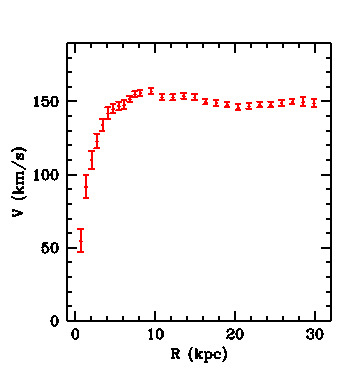
\includegraphics[width=0.5\textwidth]{images/rotation.jpg}
        \caption{From "Rotation Curves" by Martin White, UCB Department of Astronomy}
        \label{fig:rotation}
    \end{figure}
    
    %https://w.astro.berkeley.edu/~mwhite/darkmatter/rotcurve.html
    From the above diagram one can observe that the observed rotation of galaxy with respect to the radius does not follow the inverse square root trend discussed above. As the radius from the galactic centre increases the orbital speed does not decrease as much as what Newtonian dynamic suggested, instead the rotation curve flattens out after just slightly decreasing. Therefore, the observation data suggests that Newtonian dynamics does not make the correct predictions regarding to the rotation of galaxies.

    \subsection*{Dark Matter and Its Problem}
    In order to address the issue of rotation curves of galaxies, many hypothesis were made. One of the most well known and accepted is the hypothetical matter known as dark matter, which makes up around 27\% of the observable universe \parencite{noauthor_dark_nodate}. 
    %https://science.nasa.gov/astrophysics/focus-areas/what-is-dark-energy
    Furthermore, dark matter is hypothesised to be a matter that only interacts with gravity and takes up about 95\% of the mass of a single galaxy \parencite{freese_status_2017}.
    %https://ned.ipac.caltech.edu/level5/Sept17/Freese/Freese2.html
    With the non-luminous dark matter included in the mass distribution, the predicted rotation curve of a disk galaxy now has coherence to the observed rotation curve as shown in Figure 2.
    \begin{figure}[h]
        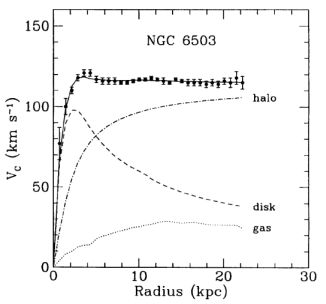
\includegraphics[width=0.5\textwidth]{images/dark_matter_rotation_curve.jpg}
        \caption{From "Status of Dark Matter in the Universe" by Katherine Freese, 2017, \textit{International Journal of Modern Physics D, 26}(6), p. 3}
        \label{fig:dm_rotation}
    \end{figure}
    %https://ned.ipac.caltech.edu/level5/Sept17/Freese/Freese2.html
    While dark matter seems to resolve the rotation curve problem, there remains several major issues with it. There is no consensus on what dark matter actually is, with hypotheses ranging from a new type of elementary particle to rogue black holes. As it does not interact with electromagnetic radiation, it has proven very difficult to detect. Ongoing major experiments involve massive underground detectors hoping to find small fluctuations that could be attributed to a dark matter particle \parencite{toomey_new_2020}. It is an incredible investment for a theory that has flushed out little-to-no details of how it works.
    
    \subsection*{Motivating MOND}
    The issue of flat rotation curves seems to point to stronger-than-expected galactic fields in the outer regions of a galaxy. The solution proposed by the dark matter hypothesis is that there is lots of extra mass in these regions, hidden from ordinary view. Another hypothesis suggests going back to first principles and rethinking gravity itself. Perhaps gravity behaves differently at galactic scales than observed at smaller ones, such as not being a true inverse-square law (Kepler's laws, of course, depend on this assumption). Certainly, this would not be the first time a new theory of gravity had to be introduced to account for unexpected observations. The primarily classical alternative to Newtonian gravity that posits to solve the problem is known as Modified Newtonian Dynamics (MOND). It is a modification of Newton's Law of Universal Gravitation that was introduced in 1982 by Israeli physicist Dr. Mordehai Milgrom \parencite*{milgrom_modification_1983}.
    %%https://articles.adsabs.harvard.edu/pdf/1983ApJ...270..365M
    Milgrom's modification of Newtonian dynamics is based on the following three assumptions:
    \begin{quote}
        (a) The force which governs the [galactic] dynamics is gravity. (b) The gravitational force on a particle depends... on the mass of the particle and the distribution of the mass which produces this force. (c) Newton's second law holds \parencite*{milgrom_modification_1983}.
        %https://articles.adsabs.harvard.edu/pdf/1983ApJ...270..365M
    \end{quote}
    The modification Milgrom proposed was to add a constant \(a_0\) which has the same dimension as acceleration being \(\mbox{LT}^{-2}\) \parencite*{milgrom_mond--pedagogical_2001}.
    %https://ned.ipac.caltech.edu/level5/Sept01/Milgrom2/Milgrom_contents.html
    This new constant is used in the MOND correction function,
    \begin{equation}
        a_N = \mu \left(\ff{a}{a_0}\right) a = \ff{GM}{r^2}
    \end{equation}
    which corrects \(a_N\), the ``Newtonian expression of acceleration" \parencite{milgrom_mond--pedagogical_2001}.
    %https://ned.ipac.caltech.edu/level5/Sept01/Milgrom2/Milgrom_contents.html
    Rather than positing that most of the mass in the universe is comprised on invisible and unknown particles, it simply states that our understanding of the dynamics of gravity are not fully captured by existing theories. It is important to note that MOND itself is a theory highly based on empirical data and currently still lacks a fundamental understanding of the correction function \(\mu\) \parencite{milgrom_mond--pedagogical_2001}.
    %https://ned.ipac.caltech.edu/level5/Sept01/Milgrom2/Milgrom_contents.html

    \subsection*{Verifying Correctness of Theories}
    The goal of this study is to simulate stellar dynamics in the Milky Way Galaxy under both classical Newtonian and MOND fields. They will be compared to each other and existing rotation curve data. Although this study does not apply MOND to make new predictions and instead focuses on determining whether it can match existing data, it remains important nevertheless. If MOND is to become an accepted theory, we must show that it can explain the phenomena we do observe before making predictions about what we haven't yet. If it can't even do that, we must reject it in its current form. Every physical theory must take this first step and that is what we aim to do here.

    
    \section*{A New Gravity}
    \subsection*{The Problems with Force Laws}
    When Newton formulated Universal Gravitation, he did it in terms of a force law, describing the gravitational force a body feels due to another. The familiar law is modified by a nonlinear correction function in Modified Newtonian Dynamics \parencite{sanders_modified_2002}.
    \begin{equation}
    F_g = \frac{GMm}{\mu(\frac{a}{a_0})r^2},
    \end{equation}
    
    where $a$ is the acceleration due to Newtonian gravity, $a_0$ is an acceleration parameter, and $\mu(\frac{a}{a_0})$ is a correction function. It has no specific definition and is ultimately found through curve fitting. The function used in this paper (known as the ``standard interpolation function") is
    \begin{equation}
    \mu\left(\frac{a}{a_0}\right) = \frac{1}{\sqrt{1 + (\frac{a_0}{a})^2}}.
    \end{equation}
    
    The problem with this force law is that, unlike Newton's Law of Universal Gravitation, it breaks conservation laws. Consider two different masses ($M \neq m$). The magnitude of the Newtonian gravitational force experienced by each is equal. With different masses, they experience different accelerations. Per (3), the two bodies would then experience different magnitudes of force under MOND, violating Newton's Third Law. As conservation of momentum and related laws are built upon Newton's Third Law, they are no longer true under MOND. Conservation laws are the bedrock of contemporary physics and theories that flout them cannot be tenable. This is not the end of MOND, however, as we show in the next section.
    
    Even if (3) did not violate conservation laws, it would still be sub-optimal to apply to a galaxy. Galaxies are extended objects, not point masses. Even though the bulk of their masses reside in individual stars, there are so many that it would be untenable to compute the force on a mass due to all the stars in the galaxy. Diffuse gas clouds are even more problematic in this sense. A galaxy is better modelled as a continuous distribution of mass. Finding the force felt by a particle from that bulk mass requires finding the galactic gravitational field, which is the realm of Gauss's Law.

    \subsection*{From Newtonian Gravity to MOND}
    ``A classical field is a dynamical system with an infinite number of degrees of freedom" and it provides the fundamental description of how matter interacts with the field \parencite{torre_introduction_2022}.
    Next, the Lagrangian of Newtonian gravity is
    %https://digitalcommons.usu.edu/cgi/viewcontent.cgi?article=1002&context=lib_mono pp13
    \begin{equation}
        \mathcal{L}(\vx, t) = - \ff{1}{8 \pi G} \left(\nabla \Phi(\vx, t)\right)^2 - \rho(\vx, t) \Phi(\vx, t) \parencite{dewar_gravitational_2018}.
    \end{equation}
    %https://core.ac.uk/download/pdf/160113562.pdf
    Note that this Lagrangian is in the form of \(\mathcal{L} = T - V\), where the kinetic energy \(T = -\ff{1}{8 \pi G} \left(\nabla \Phi(\vx, t)\right)^2\) contains the gravitational potential field since kinetic energy of the field depends on particles interaction with the potential field. (CH. Wang, personal communication, December 4, 2022) Furthermore, considering the variation with respect to \(\Phi(\vx, t)\), one can derive
    \begin{equation}
        \nabla^2 \Phi(\vx, t) = 4\pi G \rho(\vx, t),
    \end{equation}
    which is the Gauss's law for Newtonian gravity \parencite{dewar_gravitational_2018}.
    %https://core.ac.uk/download/pdf/160113562.pdf

    Next, as mentioned in an earlier section a Lagrangian approach was proposed to preserve the conservation of momentum which is equivalent to Newton's third law and resolves the issue present in the previous section. The Lagrangian for MOND is
    \begin{equation}
        \mathcal{L} = - \left(\rho \Phi + \ff{1}{8 \pi G}a_0^2F\left(\ff{\nabla \Phi^2}{a_0^2}\right)\right).
    \end{equation}
    Similar to the case of Newtonian gravity, after considering the variation with respect to \(\Phi(\vx, t)\), one will result in Gauss's law of MOND gravity:
    \begin{equation}
        4 \pi G \rho = \nabla \cdot \left[\mu \left(\ff{\abs{\nabla \Phi}}{a_0}\right)\nabla \Phi\right] \parencite{sanders_modified_2002}.
    \end{equation}
    %https://arxiv.org/pdf/astro-ph/0204521.pdf pp20
    With the Gauss's law of MOND, one can use it to find the field of MOND, which we will discuss about in our computation.

    %\subsection*{Newtonian and Deep-MOND Limits}

    %\subsection*{Simple Systems Under MOND}

    \subsection*{Coping with Nonlinearity}
    MOND is a deeply nonlinear theory. While nonlinearity allows for very interesting dynamics, it is very difficult to reconcile mathematically. It is likely that it has no analytical solutions. Computationally, partial differential equations are solved with the finite difference method (FDM), which converts a PDE into a system of algebraic equations \parencite{sauer_numerical_2017}. If the underlying equation is nonlinear, so is the algebraic system. Obtaining a good representation of the galactic field would require a very large system. Even numerically, solving such systems is difficult and prone to a host of numerical issues. Fortunately, Milgrom, one of the founders of MOND, developed a quasi-linear formulation in which the PDE is linear but the source term is nonlinear \parencite{milgrom_quasi-linear_2010}. Applying FDM would produce a linear system and the nonlinearities would be contained to the algebraic terms, a far more tractable problem. It is equivalent to the original formulation and also stems from a Lagrangian and thus preserves conservation laws. Although we do not have time for the derivation or further discussion of its nature, we present it here and proceed with it for the rest of this study.
    \begin{equation} \nabla^2 \Phi = -\div \left[v\left(\frac{|\vec{g_N}|}{a_0}\right)\vec{g_N}\right], \end{equation}

    where $\vec{g_N}$ is the Newtonian gravitational field and $v$ is a new interpolating function with the peculiar property that $v(y) = \frac{1}{\mu (x)}$ where $y = x\mu (x)$ where $x = \frac{g}{a_0}$$v(x)$ where $g$ is the ``total gravity". The meaning of these terms is beyond the scope of this study.

    \section*{Computing the Galactic Field}
        
    \subsection*{Mass Distribution of the Milky Way}
    Mass density is the source of gravitational fields. To calculate the field, we must first characterize the mass distribution of the Milky Way. One intricate model draws on a swath of observational data and careful statistical fitting \parencite{mcmillan_mass_2017}. It divides the galaxy into six components: the central bulge (6), thick and thin stellar disks (7), H1 and molecular gas disks (8), and the dark matter halo. The latter is excluded from this study. All distributions are isotropic, varying only with $r$ and $z$ in a cylindrical coordinate system centered at the center of the galaxy with $z$ axis pointing out of the galactic plane. The distributions follow equations of the following forms:

    \begin{equation}
    \label{}
    \rho_b = \ff{\rho_{0,b}}{\left(1 + \ff{r'}{r_0}\right)^\alpha} \exp{\left[ -\left(\ff{r'}{r_{\mbox{cut}}}\right)^2\right]}
    \end{equation}
    \begin{equation}
    \label{}
    \rho_d = \ff{\Sigma_0}{2z_d} \exp{\left(-\ff{\abs{z}}{z_d} - \ff{r}{r_d}\right)} 
    \end{equation}
    \begin{equation}
    \label{}
    \rho_g = \ff{\Sigma_0}{4z_d} \exp{\left(-\ff{r_m}{r} - \ff{r}{r_d}\right)} \sech^2{\left(\ff{z}{2z_d}\right)}
    \end{equation}
    \begin{equation}
    \label{}
    \text{Note: } r' = \sqrt{r^2 + \left(\ff{z}{q}\right)^2}
    \end{equation}
    Note that the two stellar discs and two gas disks obey the distribution law for each type of disk, but have different parameter values. For the sake of concision, all parameters are omitted from this paper, but can easily be found in McMillan's original paper. They are all expressed in the convenient galactic units of $\si{M_\odot}$ (solar mass) for mass and $\si{kpc}$ for space. Each density is then in $\si{M_\odot.{kpc}^{-1}}$.

    When solving Gauss's Law (for either classical or MOND fields), the sum of all these individual mass density components at a point will be used for the input term at said point. Ultimately, the field will depend on both $r$ and $z$. Considering that our primary goal is to determine how rotational speed varies with radial distance in a galaxy and that galaxies have much greater extent in their radial direction, an additional dimension is unnecessary, especially considering the added burden of numerically solving a partial differential equation in two dimensions. As such, it would be helpful to ``normalize" the distributions into being sole functions of $r$. One simple way is to find the average value of each density, centered around $z = 0$. Each density decreases exponentially along both cylindrical directions from the center. The model does not specify strict domains for its distributions. As such, we integrate the distributions until they reach a density below a certain threshold, denoting the ``edge" of the galaxy. This choice is necessarily arbitrary and a balance between capturing the entire distribution and preventing the average from being diluted by many low values at the tails. Our heuristic is the mass of the Sun. When the density is lower than one solar mass per cubic kiloparsec, the integration terminates. As a cubic kiloparsec is a huge volume, this should faithfully cover the entire galaxy as most would characterize it.
    
    The stellar and gas disks both have analytical antiderivatives.
    \begin{equation}
        \begin{aligned}
            \int_{z_i}^{z_f} \rho_b dz = &\ff{\Sigma_0}{2}e^{\left(-\ff{r}{r_d}\right)} \left(-e^{\left(\ff{z_i}{z_d}\right)} - e^{\left(-\ff{z_f}{z_d}\right)} + 2\right)
        \end{aligned}
    \end{equation}
    \begin{equation}
        \begin{aligned}
            \int_{z_i}^{z_f} \rho_g dz = \ff{\Sigma_{0} e^{\left(-\ff{r}{r_d}\right)}}{2e^{\left(\ff{r_m}{r}\right)}} \left(\tanh \left(\ff{z_f}{2z_d}\right) - \tanh \left( \ff{z_i}{2z_d}\right)\right)
        \end{aligned}
    \end{equation}
    The bulge does not. Note that the gas disk densities are undefined at $r = 0$. However, their limit is clearly $0$, so we assign them that value. We evaluate the antiderivatives at $z = -1.3 \, \si{kpc}$ and $z = 1.3 \, \si{kpc}$, corresponding to an estimate of the thickness of the Milky Way Galaxy of around $2.6 \, \si{kpc}$ \parencite{rix_milky_2013}. These values increase in magnitude by $.001 \, \si{kpc}$ every iteration, a sufficiently small size compared to the galactic scale to ensure numerical stability and accuracy. It is also an estimate for the average stellar separation in the galaxy \parencite{noauthor_what_2021}. When the difference between iterations is below our solar mass threshold, we take the present value. To evaluate the bulge integral numerically, we employ Simpson's Rule, an $\mathcal{O}(h^4)$ method \parencite{sauer_numerical_2017}. We compute the modified density every $.001 \si{\, kpc}$ starting at $r = 0$ until the total mass at a given $r$ is less than $1 \si{\, M_\odot}$, at which point it is safe to assume we have reached intergalactic space. Summing these five components give us the source of our galactic field as a function of $r$.
    
    \subsection*{Reduced Gauss's Law}
    We find the Newtonian field, required in the calculation of the MOND potential. Expanding Gauss's Law in cylindrical coordinates yields
    \begin{equation}
    \frac{1}{r}\frac{\partial(rg_r)}{\partial r} + \frac{1}{r}\frac{\partial(g_\phi)}{\partial \phi} + \frac{\partial g_z}{\partial z} = -4\pi G\rho (r).
    \end{equation}

    In galactic units, $G = 4.5171\cdot 10^{-39} \, \si{kpc^3.M_\odot^{-1}.s^{-2}}$, an absurd quantity. The mass distribution now only depends on $r$, so the partials with respect to $\phi$ and $z$ vanish. Intuitively speaking, at a given radius, the source looks the same from any azimuthal angle, so the field must be the same as well. Consider an observer at  point $(r, \, \phi, \, 0)$. At points $(r, \, \phi \pm rd\phi, \, 0)$, the mass density is the same as at the original point. The pulls in each direction are balanced out, so the field in the $\hat{\phi}$ at any point is $0$. The field is central. As the distribution is reduced to two dimensions, there is also no $\hat{z}$ component. 

    The partial differential equation then reduces to a first-order ordinary differential equation in $r$.
    \begin{equation}
    \df{(rg_r)}{r} = -4\pi rG\rho (r)
    \end{equation}
    
    This equation will be solved on a domain from $r = 0$ to some $r$ that will depend on the mass distribution. It will require appropriate boundary conditions at the endpoints to solve. Considering gravity decreases with distance, an obvious first choice is $g_r = 0$ at $r = \infty$. This cannot be truly implemented in a numerical algorithm, which requires finite quantities, but setting the field to be $0$ at sufficiently far distances from the galaxy would serve just as well. The second boundary condition is more subtle. Consider the field at $r = 0$. As the field does not depend on direction, $g$ at any point $(0 + dr, \, \phi, \, 0)$ is the same. If $g$ at $r = 0$ is equal to $g$ at these neighboring points, the radial derivative of $g$ clearly vanishes. If it is not, $g$ at $r = 0$ becomes a local extremum, which also has zero derivative. $\df{g_r}{r} = 0$, which implies that $\df{(rg_r)}{r} = 0$ as well.

    The numerical solution to (10) will be discussed in the next section. We now move onto finding the MOND potential. The correction function in the source term can be expanded as follows.
    \begin{equation}
    v(\frac{g_N}{a_0}) = \frac{1}{\mu(\frac{g}{a_0})} = \sqrt{1 + (\frac{a_0}{g})^2}
    \end{equation}
    
    We can solve for $g$ in terms of $g_N$ through the associated equations of (5).
    \begin{equation}
    \frac{g_N}{a_0} = \frac{g}{a_0}\frac{1}{\sqrt{1 + (\frac{a_0}{g}})^2} \implies g_n = \frac{g}{\sqrt{1 + (\frac{a_0}{g}})^2}
    \end{equation}
    
    Squaring both sides and rearranging yields the following quartic equation in $g$.
    \begin{equation} g^4 - g_N^2g^2 - g_N^2a_0^2 = 0 \end{equation}

    It can be verified that this quartic produces an even function with two real roots. As $g$ will be squared the sign does not matter and the equation can be solved easily through standard numerical techniques. The entire correction function becomes simply a scalar coefficient of $\vec{g_N}$, which we will denote as $a$ for concision.

    We can now expand the full source term. Recall that
    \begin{equation} \vec{g_N} = g_N\hat{r} + 0\hat{\phi} + 0\hat{z} \end{equation}

    Then 
    \begin{equation} -\div (a\vec{g_N}) = -\frac{a}{r}\frac{\partial (rg_N)}{\partial r} \end{equation}
    
    The Laplacian can be expanded as 
    \begin{equation} \nabla^2 \Phi = \frac{1}{r}\frac{\partial }{\partial r}(r\frac{\partial \Phi}{\partial r}) + \frac{1}{r^2}\ppaf{\Phi}{\phi} + \ppaf{\Phi}{z} \end{equation}

    The latter two terms vanish for the same reasons those components of the field vanish. Expanding the derivative through the product rule yields
    \begin{equation} \nabla^2 \Phi = \ppaf{\Phi}{r} + \frac{1}{r}\frac{\partial \Phi}{\partial r}. \end{equation}

    With differential and source terms expanded, Gauss's Law can be solved for the MOND potential. The same boundary conditions apply as before. As we shall see, the potential is preferable to the field for simulating stellar dynamics, so we will also find the Newtonian potential. The Laplacian is the same and the source is $4\pi G\rho (r)$, where $\rho (r)$ is the sum of the mass densities discussed earlier. 
    
    \subsection*{Finite Difference Schemes}
    The finite difference method (FDM) is the principal technique to solve boundary value problems, where the unknown function and/or its derivatives are specified along boundaries of the domain of the solution instead of just at an initial point. FDM discretizes the interior of the domain into individual points and replaces the derivative at each point with a finite difference approximation \parencite{sauer_numerical_2017}. Our domain is one dimensional: a line segment from $r = 0$ to some finite $r$. At the left boundary ($r = 0$), the derivative of the field/potential with respect to $r$ is $0$, while at the right boundary, the field/potential itself is $0$. 

    We first find the finite difference approximation to the Newtonian gravitational field. There are various ways to approximate derivatives with finite differences, each with different orders of error. We will use a second order centered difference (using two adjacent points to approximate the derivative). The unknown function is $f(r) = rg_r$. As before, the separation between points will be $h = .001 \si{\, kpc}$.
    \begin{equation} f'(r) \approx \frac{f(r + h) - f(r - h)}{2h} \end{equation}

    At a given point $(r, \, \phi, \, 0)$, Gauss's Law reads
    \begin{equation} f(r + h) - f(r - h) = -8h\pi rG\rho (r) \end{equation}
    At the rightmost point, $f(r + h) = 0$ per the right boundary condition. The left boundary is a Neumann condition. It specifies the derivative, not the function, which is itself unknown. Applying a second order forward difference (using the point itself and two points after to approximate the derivative) at the left boundary allows us to substitute in for $f(r - h)$ at the leftmost point in the FDM domain with $f'(r - h)$, $f(r)$, and $f(r + h)$.
    \begin{equation} \frac{-3f(r - h) + 4f(r) - f(r + h)}{2h} \approx f'(r - h) \end{equation}

    Recalling $f'(r - h) = 0$,
    \begin{equation} f(r - h) \approx \frac{4f(r) - f(r + h)}{3} \end{equation}

    Using $n$ points provides $n$ equations with $n$ unknowns after substituting the appropriate boundary conditions at the endpoints. This system of equations is sparse, with each equation involving at most two of the probable thousands of unknowns. That significantly reduces the computational effort required to solve it and the memory such a matrix would consume. After finding $f$, it is trivial to find $g_r$.

    Applying FDM to the potential equations under both Newtonian and MOND regimes is broadly similar, but the specific finite difference equation are different. (17) can be approximated with two finite differences, both second order in $h$.
    \begin{equation} \frac{\Phi (r + h) - 2\Phi (r) + \Phi (r - h)}{h^2} + \frac{\Phi(r + h) - \Phi(r - h)}{2rh} \end{equation}
    
    Multiplying by the common denominator and using $s$ to represent a generic source term from the original differential equation yields
    \begin{equation} (2r + h)\Phi(r + h) - 4r\Phi (r) + (2r - h)\Phi (r - h) = 2h^2rs \end{equation}

    Applying the right boundary condition results in a trivial modification to the final equation. Applying the left one once again requires a forward difference at $r = 0$. This yields the first equation in the system (at point $r = h$).
    \begin{equation} \frac{-4}{3}(r + h)\Phi (r) + \frac{4}{3}(r + h)\Phi (r + h) = 2h^2rs \end{equation}

    $s$ is straightforward for the Newtonian potential. The source for the MOND potential, however, itself requires a derivative (of the calculated Newtonian field) that must be approximated with a finite difference.
    \begin{equation} -\frac{a}{r}\frac{\partial (rg_N)}{\partial r} \approx -\frac{a}{r}\frac{(r+h)g_N(r + h) - (r - h)g_N(r - h)}{2h} \end{equation}

    At the right endpoint, $g_N(r + h) = 0$, whereas at the left endpoint $r - h = 0$, simplifying their respective formulas and sidestepping the need for substitutions with other finite difference formulas. 

    \subsection*{Implementation and Results}
    The large scale of the computations required necessitates picking a fast language. We opted for C++. The modified mass distribution is shown in Figure 3 with a semilog plot. As expected, the mass density decreases with increasing radius, although it seems to exist in two regimes. The first is out to just over $10 \, \si{kpc}$, corresponding to the approximate radius of the Milky Way \parencite{goodwin_relative_1998}. The density sharply decreases by several orders of magnitude. From there, the density declines linearly in the logarithmic domain, corresponding to exponential decay on linear scales, in line with the density equations detailed earlier. Even as the mass becomes sparser, it is not until close to $120 \, \si{kpc}$ out from the center, deep into intergalactic space, that the mass density falls below $1 \, \si{M_\odot \,kpc^{-3}}$. Whether this is a mathematical phenomenon or a reflection of an actual mass distribution is a question for another paper.

    \begin{figure}[h]
        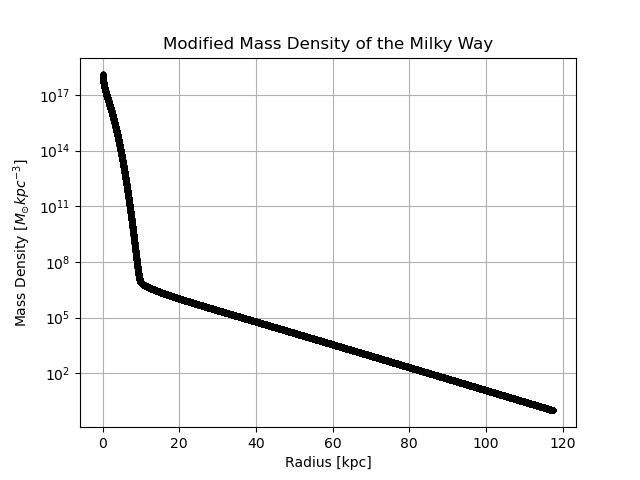
\includegraphics[width=0.5\textwidth]{images/modmass.png}
        \caption{The mass density of the Milky Way as a function of distance from the galactic center is shown. Note how the density exhibits exponential decay, albeit with two very different decay scales that transition sharply at the rough cutoff point of the galaxy.}
        \label{fig:rotation}
    \end{figure}
    
    With the mass found, we can find the field. Implementing a finite difference solver ultimately amounts to large scale matrix computations. We used the Eigen library of C++, which provides an especially efficient implementation for sparse matrices. Given that the mass distribution persists out to $~120 \, \si{kpc}$, we somewhat-arbitrarily selected a zero field boundary at $268 \, \si{kpc}$, which is about $20$ times an estimate for the radial extent of the Milky Way. Using a step size of $.001 \, \si{kpc}$ gives a $268,000$ dimensional system. After running FDM, we found that the field to decrease in a nice, continuous manner as expected for the first few $\si{kpc}$. However, starting around $6.5 \, \si{kpc}$, the fields at adjacent points jumped around, with the discontinuities growing by several orders of magnitude as $r$ increased. This persisted regardless of the absolute magnitude of the field or the distance of the boundary. It is clearly some numerical issue. In the interest of time, we accepted working within the inner $6.5 \, \si{kpc}$ of the galaxy. The field up to $6.5 \, \si{kpc}$ is shown in Figure 4, once again on a semi-log plot. It exhibits a very sharp initial decrease followed by roughly exponential decay. This exponential decay corresponds to that of the mass density. Although the reasons for the spike towards $r = 0$ are unclear, it may be due to the boundary condition enforcing a maximum there, which sharply drops off in proportional to the mass density.

     \begin{figure}[h]
        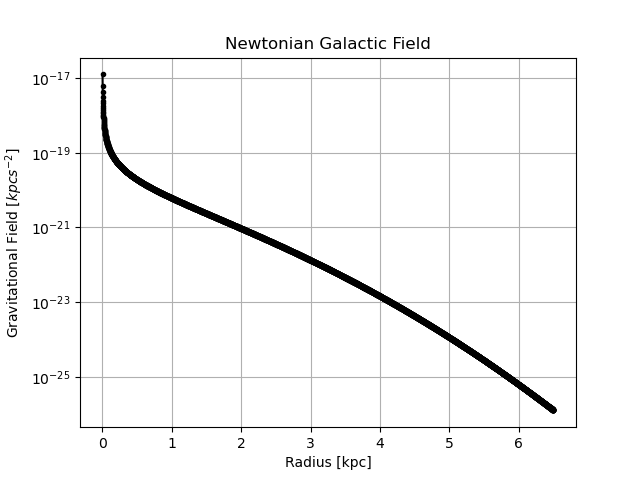
\includegraphics[width=0.5\textwidth]{images/nfield.png}
        \caption{The Newtonian gravitational field of the Milky Way as a function of radius is shown. As with the mass density, it declines exponentially, but with varying decay rates.}
        \label{fig:rotation}
    \end{figure}

    The final step is to find both Newtonian and MOND potentials for the galaxy as described above. They are plotted simultaneously in Figure 5. It is cropped at $6.5 \, \si{kpc}$ to avoid the numerical instability of the numerical field. Further discussion is reserved for a later section. 

    \begin{figure}[h]
        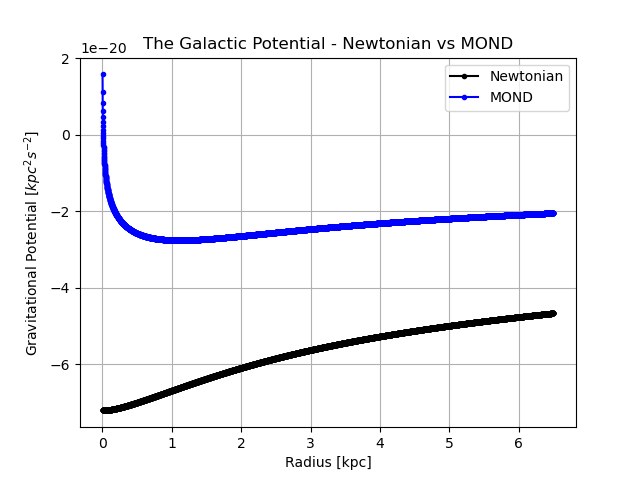
\includegraphics[width=0.5\textwidth]{images/galpot.png}
        \caption{The gravitational potentials under both regimes are shown. Curiously, the MOND potential is non-negative in the inner parts of the galaxy, indicating a potential hill, rather than a well as expected.}
        \label{fig:rotation}
    \end{figure}

    \section*{Stellar Dynamics Simulation}
    \subsection*{The Need for Symplectic Integration}
    Equipped with the gravitational potentials of the Milky Way, we turn out attention to our main goal: simulating stellar orbits to generate rotation curves. The equation of motion for a star can be written in any formulation of mechanics. That will yield an initial value problem that can be solved numerically. Runge-Kutta methods are typically used, but they can accumulate large errors when modelling dynamical systems over long time scales. A natural unit of time to use here is the galactic year, the time it takes for the Sun to orbit the galactic center, approximately 230 million years \parencite{fraknoi_how_2007}. Applying a Runge-Kutta method over that time scale would generate significant numerical drift, particularly in the total energy of the system, which is meant to be conserved. Symplectic integrators are designed specifically to conserve energies over long time scales, and, as such, are applied frequently in high-end physical simulations \parencite{donnelly_symplectic_2005}. Symplectic methods are built around Hamiltonians, as they conserve certain properties of the phase space that correspond to energy, so we will proceed with that approach.

    \subsection*{Stellar Equations of Motion}
    In this simulation, a star will be constrained to move in the galactic plane. The generalized coordinates are $r$ and $\phi$ from the aforementioned cylindrical system. The total energy is conserved and the translation from these coordinates to Cartesian is time independent, so the Hamiltonian of a star is simply its total mechanical energy.
    \begin{equation} \mathcal{H} = \frac{1}{2}m\vec{v}^2+m\Phi (r) \end{equation}

    In general, the mass of a star varies greatly, but it is always small enough to be treated as a point particle with respect to the galaxy. As it ultimately does not have a great impact on the simulation, $m$ will be set to $1 \, \si{M_\odot}$ for simplicity. 

    Expanding with velocity in cylindrical coordinates and noting that $\dot{z}$ is obviously $0$, we have
    \begin{equation} \mathcal{H} = \frac{1}{2}m(\dot{r} + r^2\dot{\phi}^2) + m\Phi (r). \end{equation}

    The Lagrangian follows simply.
    \begin{equation} \mathcal{L} = \frac{1}{2}m(\dot{r} + r^2\dot{\phi}^2) - m\Phi (r) \end{equation}

    The generalized momenta are then
    \begin{equation} \vec{p} = \frac{\partial \mathcal{L}}{\partial q} = (m\dot{r}, \, mr^2\dot{\phi}).
    \end{equation}

    Solving for the velocities and back substituting yields our complete Hamiltonian, from which we can write Hamilton's Equations.
    \begin{equation} \mathcal{H} = \frac{1}{2m}(p_r^2 + \frac{1}{r^2}p_\phi^2) + m\Phi (r) \end{equation}
    \begin{equation} \dot{\vec{q}} = \frac{\partial \mathcal{H}}{\partial \vec{p}} = (\frac{p_r}{m}, \, \frac{p_\phi}{mr^2}) \end{equation}
    \begin{equation} \dot{\vec{p}} = -\frac{\partial \mathcal{H}}{\partial \vec{q}} = (\frac{p_\phi^2}{mr^3} - m\df{\Phi (r)}{r}, \, 0) \end{equation}

    We now apply the symplectic Euler's method to solve this system. It is similar to Euler's method in that it iteratively updates the generalized coordinates and momenta with their instantaneous slopes (Hamilton's Equations). What makes it symplectic is that once a new value is computed, that updated value will be used to iterate all the values that come after \parencite{donnelly_symplectic_2005}. The equations are as follows.  
    \begin{equation}
        \ca{
        r_{i + 1} = r_i + \frac{\partial \mathcal{H}}{\partial p_r}\Delta t = r_i + \frac{p_{r_i}}{m}\Delta t\\
        \phi_{i + 1} = \phi_i + \frac{\partial \mathcal{H}}{\partial p_\phi}\Delta t = \phi_i + \frac{p_{\phi_{i}}}{m{r_{i + 1}}^2}\Delta t \\
        p_{r_{i + 1}} = p_{r_i} - \frac{\partial \mathcal{H}}{\partial r}\Delta t = p_{r_i} + (\frac{p_\phi_i^2}{m{r_{i+1}}^3} - m\df{\Phi (r)}{r})\Delta t \\
        p_{\phi_{i + 1}} = p_{\phi_i} - \frac{\partial \mathcal{H}}{\partial \phi}\Delta t = p_{\phi_i} }
    \end{equation}

    Note that one of the equations involves a derivative of $\Phi (r)$, which, as previously, will have to be approximated with a centered finite difference. These equations must be given initial conditions. $r(0)$ will be incremented from $.001 \, \si{kpc}$ to $6 \, \si{kpc}$, stopping there to avoid the numerical issues discussed earlier. In order to maximize the data generated from this simulation, an orbit will be integrated at every $.001 \, \si{kpc}$, the usual step size. As this system is symmetric, the initial value of $\phi$ does not ultimately matter, so we take $\phi(0) = 0$. The initial momenta are trickier. If a star does begins with $p_\phi = 0$, it will just fall towards a minimum potential and oscillate about it. For the stars in the Milky Way to be rotating at roughly constant radii, they must have had initial a nonzero initial  $p_\phi$. However, if they had too much, they would have escaped the galaxy. Based on empirical rotation curve data, a star has an average rotational speed of $209.2284 \, \si{km \, s^{-1}}$. The minimum in the dataset is $125.01 \, \si{km \, s^{-1}}$ and the maximum is $233 \, \si{km \, s^{-1}}$ \parencite{bhattacharjee_rotation_2014}. Although this rate ultimately depends on the star's position in the galaxy, to avoid drawn-out calculations of what this initial value ``should be" at varying $r$, we employ three simulations at each $r$, fed with $p_\phi(0) = mr^2\dot{\phi}$ for the three initial velocities given above. For simplicity, we set $p_r(0) = 0$ to ensure that any variation in radius is a result of gravitational interactions and not initial velocities.

    The natural time unit is one galactic year (gy). To minimize error, the time step will be $.00001 \, \si{gy}$, corresponding to about $2300$ Earth years. All times, velocities, and momenta will be computed in terms of galactic years. The question turns to how to extract rotation curve data from these orbit simulations. The Milky Way is mostly stable, with stars not dramatically changing their distance from the galactic center. We cannot be certain of that in our simulation. Although certainly imperfect, we decided to simulate the orbits for a very long time scale ($5 \, \si{gy}$) and take the $r$ and $p_\phi$ at that final time step. If the orbits will ever attain a steady state, it will be after such a long time scale. The orbital speed will then represent the rotation curve at the given radius. Amassing a large collection of final radii and speeds will provide a strong dataset to generate rotation curves and perform analysis. We note that the simulation is terminated if a star wanders beyond $r = 6.5 \, \si{km \, s^{-1}}$ to avoid noise being introduced into the dataset from the numerically-anomalous fields at large radii.
    
    \subsection*{Rotation Curves}
    The plot of the empirical rotation curve is shown in Figure 7. It includes data from stars extremely far out from the galaxy at almost $200 \, \si{kpc}$. This gives the overall impression of a declining rotational speed. However, note that the speeds are relatively consistent for the small left end of the graph corresponding to the core of the Milky Way, which is congruent with other observations and requires an explanation. Of course, stars cannot rotate at the same velocity indefinitely far out from a galaxy, and that is what we see here.
    
    \begin{figure}[h]
        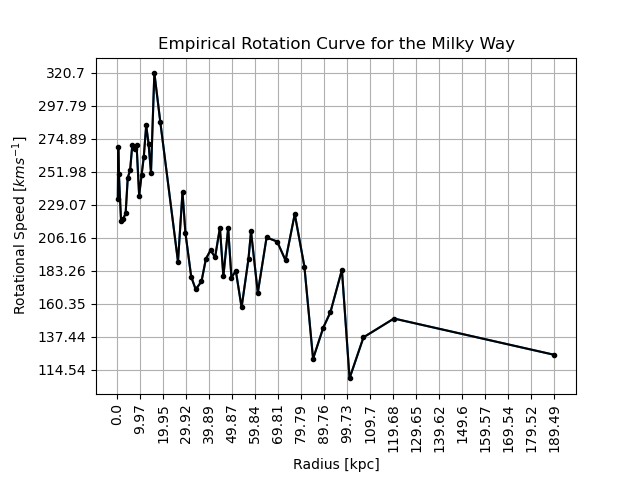
\includegraphics[width=0.5\textwidth]{images/empirical.png}
        \caption{The empirical rotation curve is shown. The rotational speeds remain rather steady until significantly beyond the reach of the galaxy, after which they collapse.}
        \label{fig:rotation}
    \end{figure}

    Now we present the results of our rotation curve simulations in Figures 8 and 9. They are lackluster to say the least. It turns out that almost all the stars, regardless of initial conditions, reached a radius of $6.5 \, \si{kpc}$, at which point the integration terminated. Very few, if any, of the data points represent a steady state orbit as evidenced by the wide range of velocities seen for $r = 6.5 \, \si{kpc}$. They really do not comprise a curve in any meaningful sense. Perhaps not terminating at a certain boundary would have alleviated this issue, but the data may have alternatively been corrupted by the aforementioned numerical error. Due to technical difficulties with Matplotlib, we were unable to plot the ``curve" for the stars in the Newtonian potential, but it experienced the same fundamental issues as the MOND orbits. No meaningful comparisons can be made with this dataset. The plot of stars with initial velocities of $209.2284 \, \si{km s^{-1}}$ is excluded as it adds no value to the discussion. Whatever can be discussed about these results is included in the next section.

    \begin{figure}[h]
        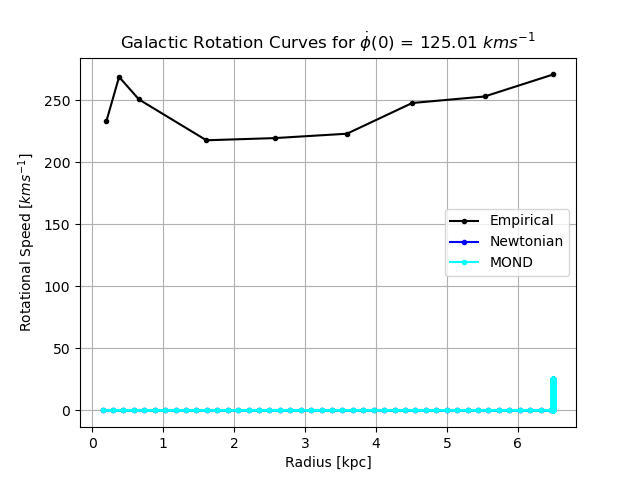
\includegraphics[width=0.5\textwidth]{images/low.png}
        \caption{The empirical and simulated rotation ''curves" are shown for the low estimate of a star's initial velocity. Clearly, the stars all sought to get to greater distances from the center of the galaxy.}
        \label{fig:rotation}
    \end{figure}

    \begin{figure}[h]
        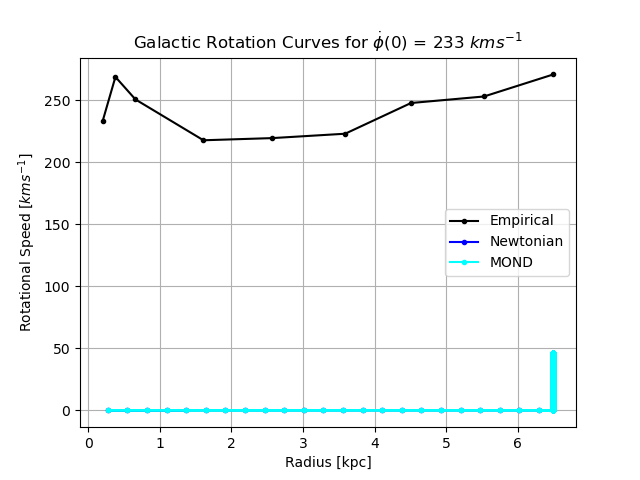
\includegraphics[width=0.5\textwidth]{images/high.png}
        \caption{The same plot as above but with a higher initial velocity is shown. The final velocities are higher than the above plot, but not much else has changed.}
        \label{fig:rotation}
    \end{figure}
    
    \section*{Analysis and Discussion}
    \subsection*{Comparison of Newtonian and MOND Potentials}
    The potentials share as many similarities as differences. The potential for both regimes was defined to be, and should be, $0$ at $\infty$. Any other point should have a negative potential. For $r > 1 \, \si{kpc}$, this is what we see. Both potentials are negative and climb gradually towards zero as $r$ increases. Interestingly, they stay within an order of magnitude throughout, contrasted with the exponential decays of the mass densities and Newtonian fields. In absolute value, the potentials are extremely different. The MOND potential is clearly far stronger than the Newtonian one. Fixing the rotation curve problem requires stronger gravitational fields. Dark matter creates extra mass to achieve this, whereas clearly MOND manages to do so without. Figure 7 shows the percentage difference between the potentials at each $r$.
    
    Perhaps the most interesting and unexpected behavior is for small $r$. The Newtonian potential continues to decrease, settling into a well at the center of the galaxy. The MOND potential does the complete opposite, achieving a maximum at the center that is so high, it is positive, resembling the potential diagram of an electron around a nucleus. This is completely unexpected. Rather than being attracted to the galactic center as in a Newtonian regime, a particle would actively be repelled from it. Repulsive gravity has no experimental basis and it is unclear whether this effect is a prediction of MOND theory here or a numerical phenomenon. Both potentials had identical boundary conditions. The MOND potential depended on the divergence of the Newtonian field, which was clearly quite high for small $r$. This could point to a flaw in our simulation setup or a problem with the version of MOND used. Further work is required here. 

    \begin{figure}[h]
        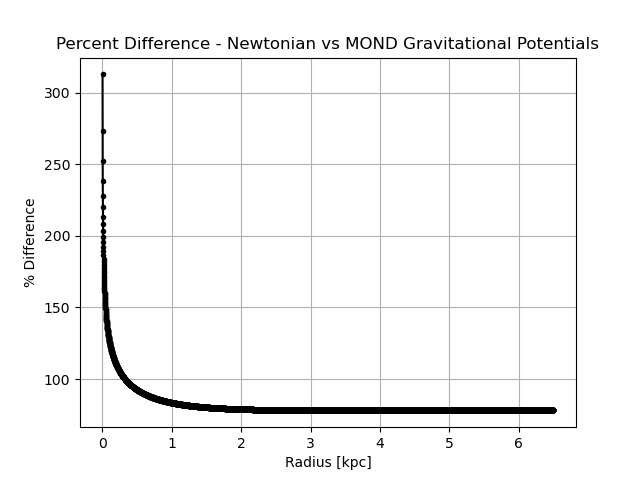
\includegraphics[width=0.5\textwidth]{images/perdiff.png}
        \caption{The percentage difference between the potentials is shown. The potentials are extremely different around $r = 0$ and gradually grow closer.}
        \label{fig:rotation}
    \end{figure}
    
    \subsection*{Comparison of Rotation Curves}
    The simulated rotation ``curves" don't provide much room for analysis. The fact that most stars, even those starting at an initial velocity experienced by a star nearly $200 \, \si{kpc}$ away, raced outwards indicates some deep problems with our simulation. It would make sense if some subset of the MOND stars starting at small $r$ raced outwards, pushed on by the positive gravitational potential. However, they even did that for the perfectly normal Newtonian field. It is still possible energy was conserved. As $r$ increases, so does potential energy, which could help explain why the speeds are so much lower than empirical data. It is worth noting that the stars with lower initial velocities (Figure 8) tended to have lower final velocities than the ones that started at higher initial velocities (Figure 9), which does agree with intuition. The lack of settling down to steady orbits shows the flaw in believing that simply running the simulation for long enough would yield good data. Rotation curve simulations are not new and there must be better ways to study them than we attempted. Ultimately, the lack of sensible data means we cannot make a conclusion on whether MOND solves the rotation curve problem.
    \subsection*{Sources of Error}
    There were many sources for error throughout this study. Prominently, the finite difference approximations used to solve for the field and potentials were second order in $h$, which is rather lackluster. The symplectic Euler method was first order. Although its energy-conserving nature should have ensured relative accuracy, at least to the extent that its inputs were accurate, higher-order methods would have been more desirable. There is also the issue of error propagation where errors introduced in earlier calculations have spiraling effects on later ones. The early issues with FDM on the galactic field constrained the rest of the program. Our entire methodology is also questionable, such as whether it makes sense to project a three-dimensional distribution into two and the entire approach to simulating rotation curves. Initial conditions are of non-trivial importance, especially in dynamical systems like a galaxy. Picking random initial velocities from empirical data is likely ill-advised and not reflective of the true dynamics of galaxies.  

    \section*{Conclusion}
    Modified Newtonian Dynamics (MOND) is an alternative classical theory of gravity that attempts to explain the rotation curve problem: why the rotational velocities of stars in galaxies does not decrease with distance as predicted by classical mechanics. Dark matter is one possible explanation, whereas MOND is another. We introduced the field equations of MOND and a specific mass model of the Milky Way and numerically found the potentials generated under both Newtonian and MOND regimes. We then integrated stellar orbits in both potentials in an attempt to generate rotation curves and evaluate the extent to which MOND solves the problem. Although we found the MOND potential to be far stronger than the Newtonian one, it exhibited anomalous behavior for small $r$. The rotation curves were mired in issues for both potentials that made them functionally unusable. Given these underlying issues, we cannot make a determination regarding whether MOND solves the rotation curve problem and an acceptable alternative theory of gravity. Future work is required. It must apply a more rigorous and sound approach to both physical analysis and numerical simulation to fix these untenable issues. It would be nice to consider a full three-dimensional space and include a simulation with Newtonian gravity and dark matter to test both theories. Furthermore, there are relativistic formulations of MOND, which could prove interesting to study galactic evolution and cosmology with. All will have to wait. If nothing else, we hope we have helped illuminate this corner of heterodox physics and inspired ourselves or others to pursue this cause further.
    
    \section*{Acknowledgements}
    We would like to thank Professor Francis Poulin for his guidance and encouragement on this project and his excellent teaching of classical mechanics. Furthermore, we would like to thank Professor Douglas Harder for his help tackling the original non-linear MOND PDE in the early stages of this project. Finally, we would like to thank University of Waterloo's Computer Science Club for providing computing services for its club members, allowing us to simulate MOND with higher efficiency.
    \section*{Citations}
    \printbibliography[heading=none]
\end{document}
